La tavola periodica fu iniziata da Mendeleev, il quale raggruppò gli elementi aventi relazioni simili. Oggi sappiamo che essa è ordinata per numero atomico crescente. È formata da linee verticali dette gruppi e linee orizzontali dette periodi.

\textbf{Elemento}: è una sostanza costituita da un solo tipo di atomi.

\textbf{Atomo}: la più piccola parte dell'elemento che conserva tutte le
caratteristiche chimiche dell'elemento stesso.

\textbf{Composto}: Sostanza formata da due o più atomi legati
chimicamente.

\(\ce{ A + B -> AB }\) composto

\(\ce{ A + A -> A2 }\) forma molecolare di A

L’equazione chimica rappresenta le trasformazioni che le sostanze subiscono. A sinistra si pongono i reagenti, a destra i prodotti. La freccia indica il verso della trasformazione. Lo stesso elemento può presentare una forma microscopica diversa. La grafite è formata da strati di atomi di carbonio che si collegano ad altri tre, formando un foglio di anelli esagonali. Il diamante è formato da anelli esagonali di carbonio non disposti su un piano. Esse sono due forme allotropiche del carbonio.

\begin{figure}[htp]
    \centering
    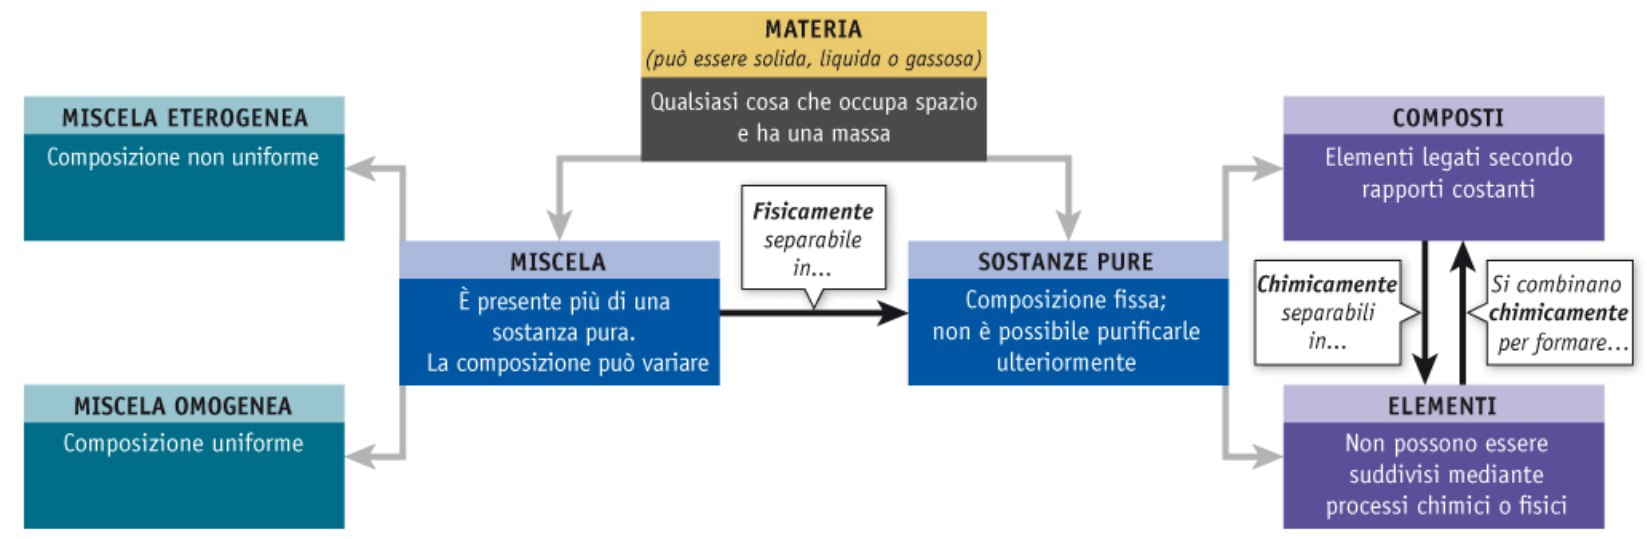
\includegraphics[width=18cm]{immagini/materia.jpg}
\end{figure}

Tre sono le leggi fondamentali che regolano l'andamento delle reazioni chimiche:

1. \textbf{Legge della conservazione della massa}: durante le reazioni chimiche la quantità di massa è invariabile.

2. \textbf{Legge dell'invariabilità delle sostanze elementari}: non si può trasformare un elemento in un altro \(\ce{ A -> B }\) MAI.

3. \textbf{Legge delle proporzioni definite}: ogni composto ha una composizione costante, cioè contiene sempre gli stessi elementi secondo rapporti definiti e costanti, caratteristici del composto.

\textbf{Numero atomico} (Z): numero di protoni di un atomo.

\textbf{Numero di massa} (A): somma dei numeri di protoni e neutroni di un
atomo.

\textbf{Isotopi}: atomi con lo stesso numero atomico ma diverso numero di
massa (stesso numero di protoni ma diverso numero di neutroni).

La \textbf{massa atomica} M ($\neq$ dal numero di massa A) è la massa di un dato atomo. La massa atomica assoluta viene espressa in chilogrammi: l'ordine di grandezza dei valori è $10^{-25}-10^{-27} kg$. Per ovviare alla scomodità di avere nei calcoli numeri così piccoli, si è convenuto di esprimere la
massa atomica in rapporto alla massa atomica assoluta di 1/12 dell'atomo \(\ce{ ^{12}C }\), il cui valore è adottato nel SI quale unità di massa atomica (\textbf{uma}): sperimentalmente equivale a 1.66053886$\cdot
10^{-27} kg$. (Quindi 1 uma$\sim$massa di un protone$\sim$massa di un neutrone)
La \textbf{massa atomica relativa} (o \textbf{peso atomico} (mortacci vostra e di chi non ve lo dice)) vale:
$$m_{rel}=\frac{m_{ass}}{1 u}=\frac{m_{ass}}{1.66053886\cdot
10^{-27} kg}$$
La massa atomica relativa (adimensionale) è legata al numero di nucleoni presenti nell'atomo.

Il numero di atomi presenti in 12 grammi esatti di \(\ce{ ^{12}C }\) è pari a $6.02214076\cdot10^{23}$ (costante di Avogadro [mol$^{-1}$]).

Protoni e neutroni hanno massa leggermente diversa ( differenza 2 per mille). La massa assoluta degli atomi è leggermente inferiore alla somma delle masse delle particelle che li compongono perché parte della massa delle particelle che costituiscono il nucleo è stata trasformata in energia di legame dei nucleoni (difetto di massa).
La massa degli elettroni incide poco perché è pari a 1/1836 quella del protone.

La massa assoluta si può calcolare solo effettuando una misura, ad esempio con lo \textbf{spettrometro di massa}. Il campione vaporizzato da analizzare è introdotto nella camera di ionizzazione in cui gli elettroni strappano elettroni dagli atomi del campione che poi vengono accelerati da ddp ed infine un campo magnetico li fa curvare con raggio di curvatura proporzionale a massa/carica.

Analogamente si definisce anche la \textbf{massa molecolare relativa} (o \textbf{peso molecolare}). Per esempio, se avessimo un composto di formula \(\ce{ A2BC3 }\)A, il suo peso molecolare sarebbe dato da:
$$p.m.= 2\cdot p.a.(A) + p.a.(B)+ 3\cdot p.a.(C)$$
Anche piccolissime quantità di sostanze contengono un gran numero di atomi.
Sono state concepite delle unità per esprimere numeri di tali ordini di grandezza e per avere quantità con le quali poter lavorare agevolmente in laboratorio.

\textbf{Grammo atomo} = massa in grammi eguale al peso atomico (o 
massa atomica relativa)

\textbf{Grammo molecola} = massa in grammi eguale al peso molecolare (massa molecolare relativa)

\textbf{Grammo atomo o Grammo molecola} = mole ($\leftarrow$ sono inutili)

Riassunto: Una mole di qualcosa contiene un numero di grammi pari alla massa atomica/molecolare relativa  di quel qualcosa (molecola,  atomo, ione). Una mole di ossigeno pesa 16 grammi (l'ossigeno ha massa atomica relativa = 16). Ah e alla fine grammo atomo e grammo molecola non servono a niente visto che si usano le mole oggi.

Una mole di oggetti contiene un numero di oggetti uguale a quello degli atomi di carbonio presenti in 12 g esatti di \(\ce{ ^{12}C }\). = n. di Avogadro.

Il numero di moli di un composto/elemento vale
$$n=\frac{\text{grammi di composto/elemento}}{\text{massa atomica/molecolare relativa}}$$
Le formule chimiche ci dicono quali elementi sono presenti nei composti e quale è il rapporto tra essi. Ma non ci dice come sono disposti nello spazio, per quello esistono le formule di struttura che mostrano i legami.
\begin{figure}[htp]
    \centering
    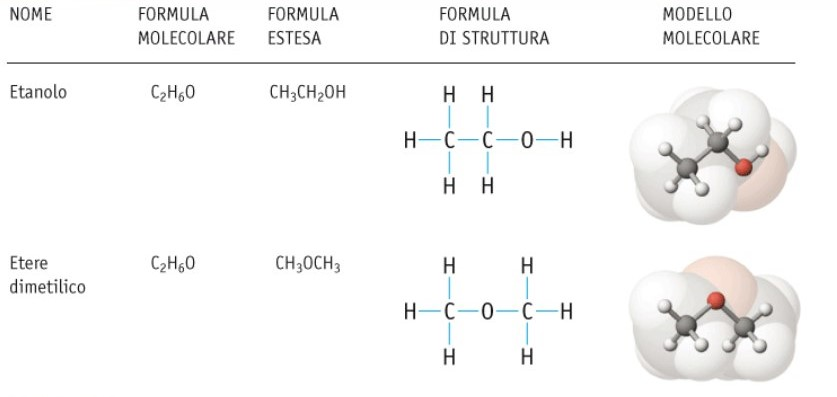
\includegraphics[width=18cm]{immagini/formula.jpg}
\end{figure}\\